\documentclass[openany,a5paper,16pt]{mystyle}

%----------------------------------------------------------------------------------------
% Linguagem: português brasil
\usepackage[utf8]{inputenc}
\usepackage[T1]{fontenc} 
\usepackage[brazilian]{babel}
\usepackage{hyphenat}
\hyphenation{mate-mática recu-perar}
\usepackage{lipsum}

%----------------------------------------------------------------------------------------
% Caixas de texto
\usepackage[most]{tcolorbox}
% Cores do livro
\definecolor{myred}{RGB}{178, 85, 56}
\definecolor{myblue}{RGB}{120,149,164}
\definecolor{myocre}{RGB}{109,82,23}
\definecolor{ocre}{RGB}{120,149,164}
\definecolor{mygrey}{RGB}{65,64,66}

\newtcolorbox{ficadica} {
    enhanced jigsaw, height = 40mm, height plus = 120mm, colback=white,colframe=myocre,coltitle=myocre,
    sharp corners, detach title, leftrule=26mm,
    underlay unbroken and first={
        \node[below,text=white,font=\bfseries,align=center]
            at ([xshift=-13mm,yshift=-1mm]interior.north west) {Fica a Dica}; 
        \node[align=center] 
            at ([xshift=-13mm, yshift=12.5mm]interior.south west) {
\includegraphics[width=26.2mm]{img/saibamais.png}};
    },
}

\newtcolorbox{saibamais} {
    enhanced jigsaw, height = 40mm, height plus = 120mm, colback=white,colframe=myblue,coltitle=myblue,
    sharp corners, detach title, leftrule=26mm,
    underlay unbroken and first={
        \node[below,text=white,font=\bfseries,align=center]
            at ([xshift=-13mm,yshift=-1mm]interior.north west) {Saiba mais}; 
        \node[align=center] 
            at ([xshift=-13mm, yshift=12.5mm]interior.south west) {
\includegraphics[width=26.2mm]{img/definicao.png}};
    },
}

\newtcolorbox{atencao} {
    enhanced jigsaw, height = 40mm, height plus = 120mm, colback=white,colframe=myred,coltitle=myred,
    sharp corners, detach title, leftrule=26mm,
    underlay unbroken and first={
        \node[below,text=white,font=\bfseries,align=center]
            at ([xshift=-13mm,yshift=-1mm]interior.north west) {Atenção}; 
        \node[align=center] 
            at ([xshift=-13mm, yshift=12.5mm]interior.south west) {
\includegraphics[width=26.2mm]{img/importante.png}};
    },
}

\title{Segurança Digital}
\author{Wagner Clemente Coelho Batalha \and João Paulo Vaz Mendes}
\date{\today}

\chapterspaceabove{50mm} % Default whitespace from the top of the page to the chapter title on chapter pages
\chapterspacebelow{60mm}
\chapterimage{img/chapter_image.pdf}

\bibliography{bibliography}

%%%%%%%%%%%%%%%%%%%%%%%%%%%%%%%%%%%%%%%%%%%%%%%%%%%%%%%%%%
% Conteúdo %%%%%%%%%%%%%%%%%%%%%%%%%%%%%%%%%%%%%%%%%%%%%%%
%%%%%%%%%%%%%%%%%%%%%%%%%%%%%%%%%%%%%%%%%%%%%%%%%%%%%%%%%%
\begin{document}

\titlepage 
	{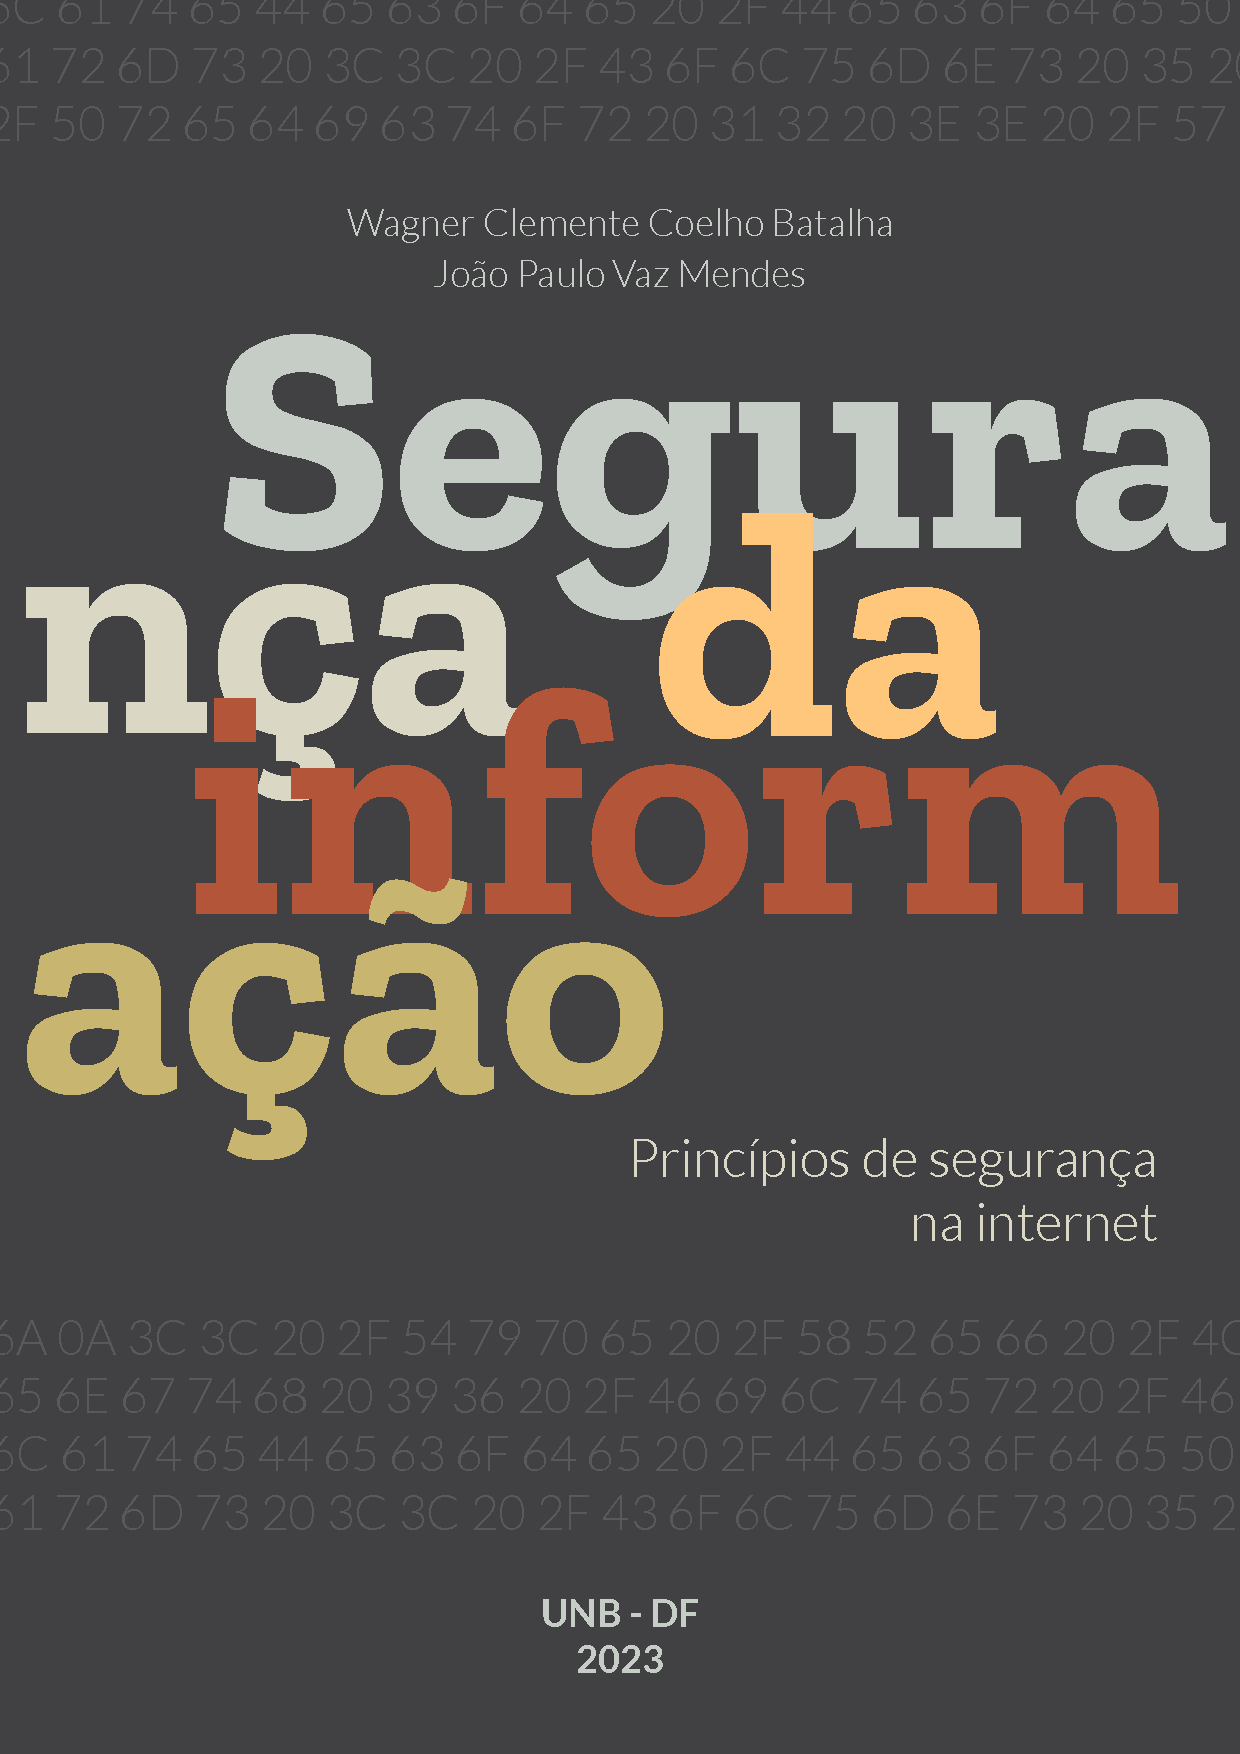
\includegraphics[height=\paperheight]{img/title.pdf}}

\tableofcontents

\chapter{Introdução}
    Alguns dos elementos que serão utilizados ao longo desse material
\begin{ficadica}
    Esta seção traz dicas relevantes para a vida das pessoas relacionadas à matéria passada
\end{ficadica}
\begin{saibamais}
    Esta seção traz algumas curiosidades com alguns detalhes interessantes para a matéria sendo um elemento a mais
\end{saibamais}
\begin{atencao}
    Esta seção traz alguma informação muito importante em relação ao conteúdo que merece destaque
\end{atencao}

\part{Noções Básicas}

\section{Introdução do Capítulo}

Neste capítulo vamos falar sobre o porquê, para começo de conversa, devemos saber como nos proteger no mundo digital. Também vamos explicar o básico para que você consiga entender diversos conceitos com mais facilidade nas próximas páginas do livro.

\chapter{Princípios}

\section{A Informação}

A Sociedade global está passando por uma alta evolução tecnológica. Carros estão começando a se dirigir sozinhos, drones estão praticamente em toda gravação na indústria cinematográfica, O GPS do celular baixa o mapa de qualquer cidade que você está e te mostra o caminho até o lugar que você quiser e até mesmo aparelhos mais inusitados como sua geladeira podem estar conectados na internet é um fato do mundo de hoje. Todas essas coisas geram, buscam ou interpretam \textbf{informação}, uma coisa que virou uma grande riqueza no mundo globalizado.

Basta você ver qualquer documento de Termos de Serviços online que você lê (Ou deveria ler) quando se inscreve em algo na internet. Em muitos deles é dito que as suas informações produzidas no serviço são utilizadas para aprimorar ele mesmo, ou então para "oferecer propagandas mais relevantes", ou até são vendidas para outras empresas que usam estes dados para diversas outras coisas. As suas informações de uso de um app, detalhes que você coloca em um post de uma rede social produzem riquezas para outras pessoas. 

A importância da informação na verdade já existe há centenas de anos. A espionagem praticamente existe há séculos para poder obter uma vantagem militar, uma fofoca no emprego pode ser usada para conseguir um aumento no salário, atrapalhar um colega chato, ou descobrir a fórmula secreta de outra lanchonete para fazer um sanduíche melhor. Tudo isso consiste em conseguir (seja de forma moral ou imoral) uma informação que vai ser preciosa para você.

Há, portanto, um conflito de interesses. A privacidade não é um direito da pessoa? Como ela vai conseguir se proteger? No Brasil a \textbf{LGPD} (Lei Geral de Proteção de Dados \cite{lgpd}), que será comentada mais adiante, protege a privacidade do brasileiro. Na outra direção, diversas empresas e sociedades buscam proteger suas próprias informações, estabelecendo regras para seus empregados e investindo em segurança.

\begin{figure}[htb]
    \centering
    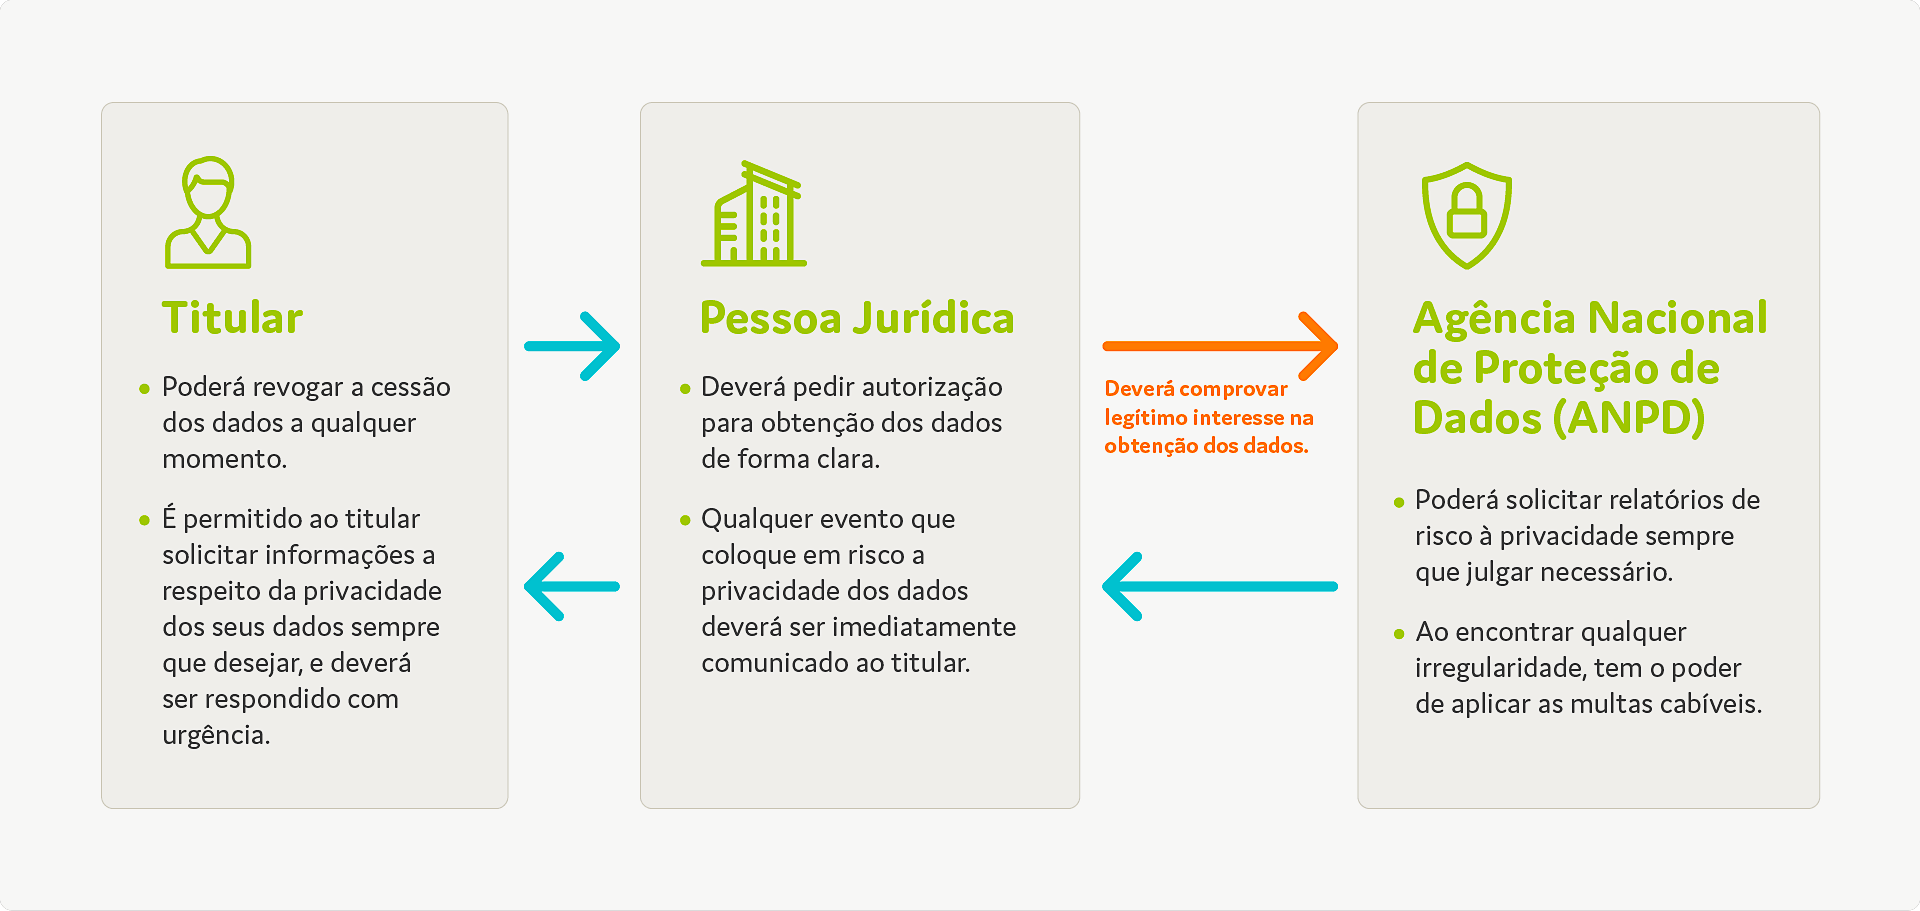
\includegraphics[width=\textwidth]{img/lgpd.png}
    \caption{Alguns dos direitos oferecidos pela LGPD. Fonte: \cite{senior}}
    \label{fig:lgpddireitos}
\end{figure}

\subsection{A Segurança}

Todo mundo tem algo que quer proteger. Com a informação é a mesma coisa. O termo "Segurança da Informação" é bem abrangente e pode ser definido de diversas formas. O vazamento de dados pode ser uma tragédia, trazendo prejuízos tanto a uma pessoa física, quanto a uma empresa.

Na revolução industrial a segurança da informação era pouco pensada como é hoje. Para se ter acesso aos dados de uma fábrica você precisava ir fisicamente nela e roubar documentos reais que provavelmente ficavam relativamente bem guardados. Hoje em dia as empresas tem bancos de dados digitais que podem ser acessados em qualquer ponto no globo desde que você saiba a forma correta de acessá-lo. Dado o tamanho de muitas dessas bases de dados é possível imaginar que levaria muito tempo para conseguir todas, mas não. Os dados digitais tem muita flexibilidade e em pouco tempo uma cópia completa de muitos gigabytes pode ser produzida e colocada em um pen-drive. Proteger esses dados é um investimento que muitas empresas fazem (ou deveriam fazer).

Para uma pessoa normal esse tipo de segurança se traduz em proteger as suas senhas como a do banco ou a de uma rede social. Além de levar em consideração o que a pessoa oferece ou coloca de informação na internet um outro aspecto deve ser observado: O que a pessoa consegue de informação na internet. Fake news e alguns métodos de ataques cibernéticos dependem da falta de conhecimento ou ignorância do funcionamento do mundo digital.


\subsection{Segurança da Informação}

Existe uma norma internacional de proteção da informação, a ISO/IEC 17799, que define os seguintes princípios

\begin{itemize}
    \item Confidencialidade: Somente pessoas autorizadas podem acessar informações, ou seja, houve uma permissão de acesso.
    \item Disponibilidade: Garante o acesso à informação na mesma hora para quem for acessá-la. Ou seja, o sistema e a rede que oferece esses dados deve funcionar perfeitamente.
    \item Integridade: As informações não podem ser adulteradas, no sentido de terceiros mal intencionados mudando dados para se favorecer.
\end{itemize}

Também temos que considerar que os dados produzidos devem ser legais e autênticos, ou seja, os dados foram produzidos obedecendo as leis e que quando comunicados ou enviados essas informações não foram alteradas no meio do caminho.

Em uma empresa esses princípios são observados pelo setor de Segurança da informação. Ele irá interagir com quase todos os outros setores da empresa exigindo que regras sejam observadas.

A mesma idéia pode ser usada para uma pessoa. Definindo regras e seguindo observações, ela terá poucos problemas relacionados a vazamento de dados.


\section{Incidentes de segurança}

Para explicar a violação de segurança precisamos entender o que é um Ativo. O Ativo é qualquer coisa que tenha valor para alguém e caso ele seja roubado ou violado teremos impactos negativos. É um termo bem abrangente, sua carteira é um ativo, pessoas podem ser também, seu celular, uma garrafa térmica de café etc..

A violação de segurança vai afetar negativamente o nosso ativo e essa violação pode se dar de diversas formas. Uma má operação, um ataque cibernético, desastres, falhas, são todas ameaças aos nossos ativos. Reconhecer ameaças e tentar evitá-las é uma grande tarefa.

Sabendo disso podemos começar a entender o que são ameaças à informação.

\subsection{Ameaças}

\begin{figure}[htb]
    \centering
    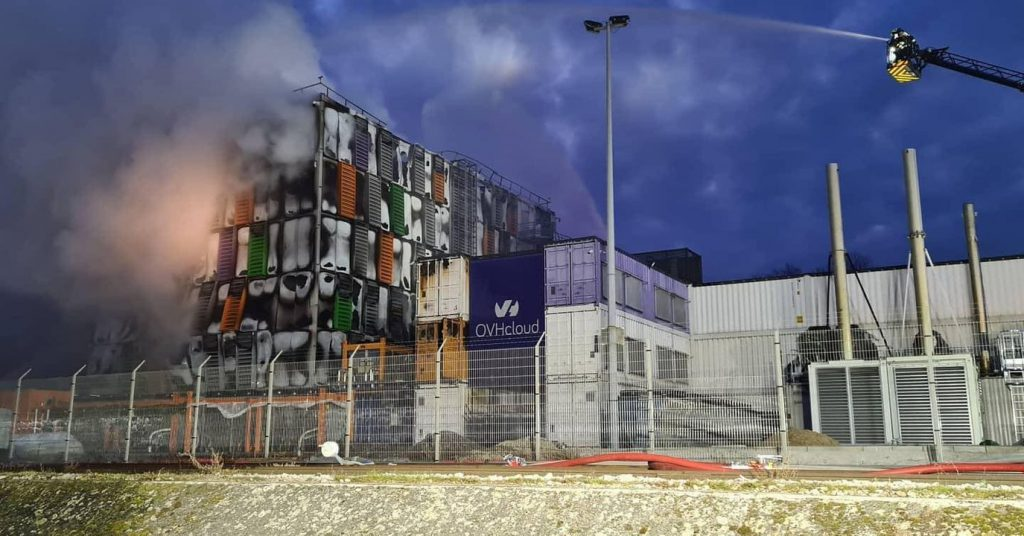
\includegraphics[width=\textwidth]{img/incendio.jpeg}
    \caption{Imaginar seu computador pegando fogo pode ser algo engraçado, mas é algo que pode acontecer. Este data center na França não teve tanta sorte e 3,6 milhões de sites ficaram fora de ar. Fonte:\cite{incendio}}
    \label{fig:incendio}
\end{figure}

Uma vulnerabilidade a um ativo da informação pode se dar das formas citadas antes, má operação, ataque, desastre, etc... E podemos separá-las em duas categorias:

\begin{itemize}
    \item Físico: Ameaças realmente físicas. Terremotos, incêndios, descargas elétricas, entre outras, nos computadores ou servidores de uma instituição;
    \item Lógico: Ameaças no mundo virtual: Vazamento de senhas, malwares, ransonwares, sites fingindo ser outros, etc...
\end{itemize}

\begin{figure}[htb]
    \centering
    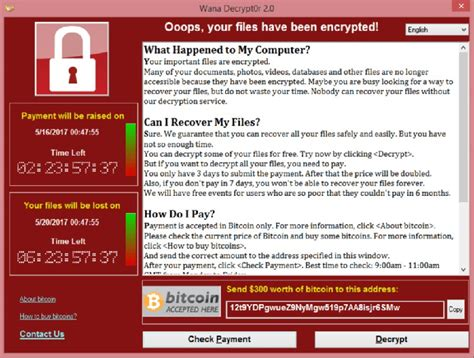
\includegraphics[width=\textwidth]{img/wannacry.jpg}
    \caption{Screenshot de um vírus de computador que ficou famoso. Esse é um tipo de vírus chamado ransonware, que encripta os arquivos pessoais do computador e exige um pagamento anônimo em criptomoeda para desencriptar.}
    \label{fig:wannacry}
\end{figure}

A forma com que se dão também podem se dividir em outras categorias:

\begin{itemize}
    \item Natural: Terremotos, tempestades, raios, enchentes
    \item Involuntárias: Ameaças inconsistentes. Acidentes de trabalho, alguém tropeçando em um fio importante, clicando um botão que não devia. Em resumo: o ator do incidente não teve a intenção de causar problemas.
    \item Intencional: Alguém quis causar problemas. Esses podem ser espiões, criminosos, invasores ou até mesmo alguém que não tenha nenhuma razão em especial.
\end{itemize}

\subsection{Vulnerabilidade}

Qualquer falha que o sistema possui e que pode dar problema. Digamos que você escreva suas senhas em um caderno. Se você deixa o caderno na cozinha existe a possibilidade de cair alguma bebida em cima dele e estragar todas suas anotações. Se você anota a senha no próprio computador em um arquivo de texto um malware pode abrir o arquivo.

Vulnerabilidades também incluem as sociais. Essa é a mais difícil de explicar e analizar já que depende do fator psicológico e emocional de uma pessoa.

\begin{figure}[htb]
\begin{ficadica}
    \subsubsection*{Golpes}
    Um exemplo de golpe que ficou comum para roubar o cartão de crédito das pessoas é a seguinte: Alguém que se diz ser do banco te liga avisando que o seu cartão de crédito foi clonado e que um motociclista vai na casa sua casa buscar o cartão para supostamente cancelá-lo e destruí-lo em segurança. Nisso ele te pergunta onde você mora para "confirmar" a sua identidade e o motociclista aparece minutos depois. Você dá o cartão para o motociclista e ele vai embora. O que você não sabia é que o motociclista e o atendente não eram do banco e agora roubaram seu cartão.

    Esse tipo de ação abusa do psicológico de um indivíduo. No início da ligação o criminoso já tenta encontrar uma vulnerabilidade através do medo: "Seu cartão foi clonado" e logo em seguida oferece uma solução: "Nós vamos na sua casa buscar seu cartão para cancelá-lo e destruí-lo". Esse tipo de ataque emocional está presente em quase todos os tipos de golpes. Outro fato que eles abusam é da falta de conhecimento, o banco nunca irá na sua casa nem irá pedir informação que já sabe. Se o banco precisa fazer algo ele fará imediatamente sem exigir nada de você.
\end{ficadica}
\end{figure}

\section{Controle de Acesso}

\begin{figure}[hb]
    \centering
    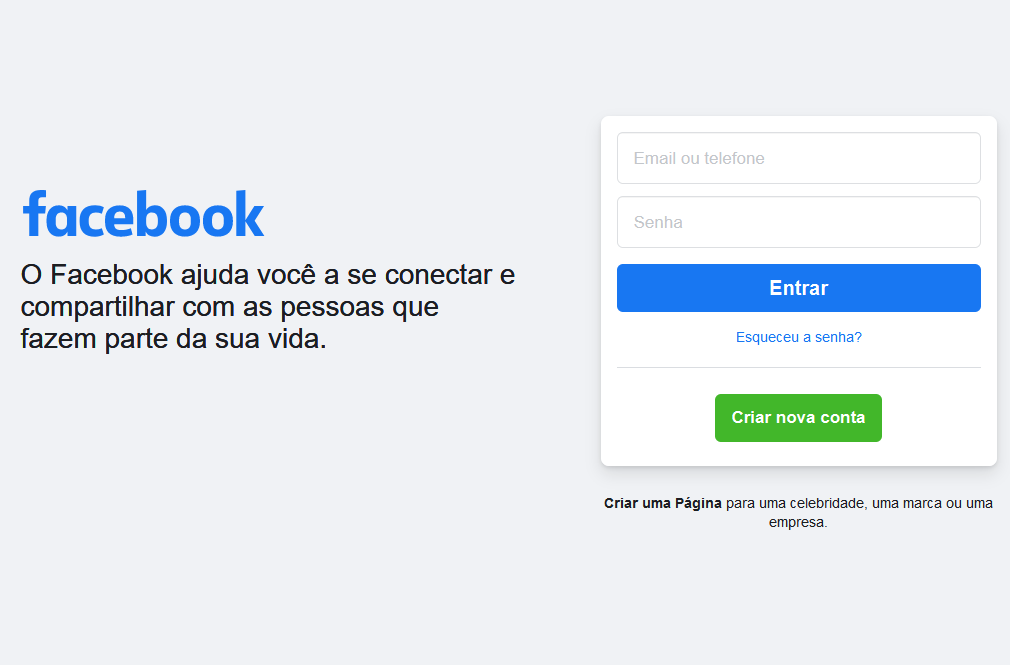
\includegraphics[width=\textwidth]{img/facebook.png}
    \caption{A página de login do facebook, exigindo seu email e senha.}
    \label{fig:facebook}
\end{figure}

Os mecanismos de segurança se baseiam em reconhecer a pessoa que quer acessar a informação. Ela se reduz basicamente a dois conceitos que tornam isso possível:

\begin{itemize}
    \item Algo que só você sabe
    \item Algo que só você tem
\end{itemize}

\subsection{Algo que só você sabe}

Esses são basicamente as senhas e perguntas que você faz a uma pessoa para identificá-la. Se alguém que quer se autenticar oferece corretamente a senha ou as respostas das perguntas que você faz a ela, você sabe que é quem diz ser.

Perguntas e respostas são um método bem rudimentar, já que alguém pode escavar a informação e descobrir resposta. Senhas também não são a melhor coisa do mundo. Senhas grandes são difíceis de memorizar e senhas pequenas são fáceis de serem descobertas. É tentador usar a mesma senha para tudo, só que se você fizer isso estará colocando todos os ovos na mesma cesta, e criando uma vulnerabilidade. 

% TODO: colocar referência ao cap 3
Falaremos mais de senhas no capítulo 3.

\subsection{Algo que só você tem}

Isto é, algo único que você tem. O que vem mais a mente é as digitais. Sua digital é praticamente única e um leitor de digital é extremamente prático em diversas situações. Pode ser usado outros tipos de identificação biométrica como a de iris e a de rosto inteiro.

Outro tipo de identificação dessa forma é a do seu celular, muito usado em autorização em duas etapas. Seu celular tem um número de série único, IMEI único e outros tipos de identificação de hardware que podem ser utilizados para sua verificação.

\begin{saibamais}
\subsection*{Hardware}

A parte eletrônica e física real do computador ou celular. São as peças que compõe a máquina, telas, caixas de som, processadores, drives, baterias, etc... \\

\subsection*{Software}

Os Software são os programas de computador. Eles não existem fisicamente e comandam o computador. É composto de todas as sequências e instruções digitais que dirigem a forma com você interage com a máquina. É armazenado digitalmente, muitas vezes no próprio computador que o utiliza.

A palavra vem do inglês, sendo um trocadilho com Hardware, onde o hard (Que significa rígido, forte) é trocado por soft (Macio). Como ware significa ferramenta, software traduz para: "Ferramenta Macia".

\end{saibamais}

\subsection{Ambos}

Uma combinação de ambos os métodos acima é ideal para sua proteção. Muitos sites oferecem, e até exigem, que você use os dois, o chamado de \textbf{Verificação em duas etapas}. Vai ser muito difícil alguém conseguir as duas formas de verificação ao mesmo tempo se você usá-la. Se alguém descobrir sua senha ainda vai precisar de seu celular para conseguir entrar na sua conta, e se ela roubar seu celular ainda vai precisar descobrir a sua senha, portanto é uma forma bem resiliente de proteção.

\section{Conclusão}

Neste capítulo vimos a importância da privacidade e da necessidade de protegê-la. Também vimos como categorizar e identificar vulnerabilidades e ameaças de segurança. No final identificamos o que torna algo seguro através de reconhecer as formas de identificação confiável através de algo que você sabe e algo que você tem.

\chapter{Exercícios}

\subsection*{Exercício 1}

Responda as perguntas abaixo:

\begin{enumerate}
    \item Porquê a noção da privacidade é necessária?
    \item Qual é a lei que oferece no brasil os direitos de proteção de dados? O que ela tem como fundamentos?
    \item Quais são os tipos de vulnerabilidade? Cite exemplos de vulnerabilidades digitais fáceis de se tomar preucauções.
\end{enumerate}

\subsection*{Exercício 2}

Marque verdadeiro ou falso nas questões abaixo:

\begin{enumerate}
    \item ( ) Incêndio causado por falha elétrica é considerado uma causa natural.
    \item ( ) Vírus de computador são ameaças do tipo lógicas.
\end{enumerate}

\part{Tudo sobre senhas}

\section{Introdução do Capítulo}

Neste capítulo vamos falar sobre uma das principais formas de proteger seus conteúdos no meio digital: as senhas. Vamos falar sobre como elas funcionam, o que elas são, como criá-las e armazená-las.

\chapter{Como Funcionam as senhas}

A senha é apenas uma das formas de acesso a um conteúdo restrito. Eles são classificados em: Algo que a pessoa possui; Algo que a pessoa é; e algo que a Pessoa Sabe. Algo que a pessoa possui é um objeto físico que se traduz digitalmente para garantir algum acesso, exemplos são Cartões de Banco, Crachás, ou tokens de acesso. Algo que a pessoa é são elemento físicos biométricos para acesso, como sensor de digitais dos dedos, ou de voz. Por fim, temos Algo que a Pessoa sabe, este é um conhecimento combinado para o acesso que se manifesta em perguntas pré-definidas, mas principalmente em senhas.
\begin{figure}[h]
\centering

\includegraphics{img/formas_de_acesso.png}
\end{figure}

As Senhas portanto são chaves para acesso a determinado ambiente virtual ou físico restrito, ou então códigos que permitem a decodificação de alguma criptografia por meio de um conhecimento específico de alguma pessoa.

O funcionamento de senhas em si funciona a partir de uma equivalência de caracteres armazenados por um registro feito anteriormente com os caracteres fornecidos quando se tenta acessar um ambiente restrito. Estes caracteres podem ser do alfabeto (a, A, z, Z), Numéricos (1, 3, 0), ou caracteres especiais (*, \&, \#). Uma vez que há um número limitado de caracteres existentes para se criar senha e também um tamanho limite de caracteres para se fazer uma senha, há a possibilidade da senha ser descoberta por alguém que não a criou se todas as possibilidades forem tentadas a exaustão. A isso, damos o nome de ataque de força bruta. Este ataque normalmente é feito com um programa de computador tentando todas as combinações possíveis de caracteres e sua quantidade nas senhas. É muito mais comum que as senhas sejam feitas apenas com letras, ou letras e números, reduzindo-se a complexidade delas, fica mais fácil a descoberta a partir do ataque de força bruta. Portanto quando se utiliza letras, números e caracteres especiais a segurança da senha é aumentada. O cálculo para a descoberta de uma senha por ataque de força bruta.

Façamos os cálculos da quantidade de possibilidades de senhas:
Com uma senha com número \textit{n} de caracteres e a ordem dos caracteres importarem devemos calcular a quantidade de possibilidades de senhas (\textit{s}) com o número de caracteres exponenciado à quantidade de caracteres (\textit{q})
\[s = n ^q\]
Para comparação podemos usar uma senha com 8 caracteres.
Considerando-se uma senha apenas de letras: Temos 26 letras no alfabeto, porém caracteres maiúsculos e minúsculos são considerados diferentes então temos \(26 . 2 = 52 \) teremos então \(s = 52^8 = 5,3 . 10^{13} \) de possibilidades de senhas a serem feitas, ou seja 53 trilhões de possibilidades. Um algoritmo de Força Bruta resolve essas tentativas em 49 minutos.

Quando adicionamos números teremos mais 10 caracteres então \( 10 + 52 = 62 s = 62^8 = 2,8 . 10^{14} \) 218 trilhões de possibilidades, com um algoritmo de Força Bruta o tempo de resolução sobe para 4 horas.

\begin{figure}[h]
\centering
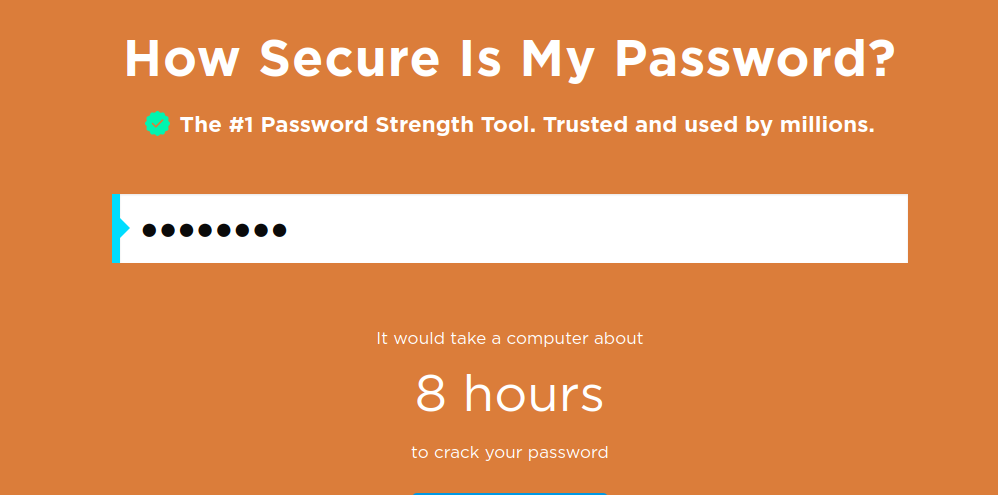
\includegraphics[width=\textwidth]{img/tempo_decifrar_senha.png}
\end{figure}


Adicionando-se a isso os caracteres especiais colocamos à soma mais 30 caracteres. \( 30 + 62 = 92 s = 92^8 = 6,6 . 10^{15} \) 6,6 quatrilhões, resultando em um tempo de 5 dias para se conseguir a senha em um algoritmo de força bruta.

Notamos uma boa diferença na segurança da senha adicionando todos os tipos possíveis de caracteres, mas também aumentando o número de caracteres temos um grande aumento de segurança. No caso de uma senha só com letras temos um aumento de 49 minutos de resolução para 92 dias de resolução utilizando 10 caracteres, ao invés de 8. Analisando uma senha com todos os tipos de caracteres temos um tempo de 5 dias de resolução com 8 caracteres e 105 anos para resolver com 10 caracteres.

/(Adicionar tabela aqui)

Porém esta não é a única forma de se conseguir descobrir uma senha. Outro ataque comum à segurança de senhas é o chamado Ataque de Dicionário que usa um banco de palavras para tentar encaixar nas tentativas exaustivas de correspondência com a senha. Tal tipo de ataque fragiliza senhas que usam as palavras mais comumente usadas em senhas extraídas de bancos de dados comprometidos e também de forma mais pessoal fica mais frágil utilizar informações pessoais facilmente encontradas de forma pública, uma nome de filho, animal de estimação, time que torce ou datas especiais podem ser utilizadas para tornar um Ataque de Dicionário mais eficiente.

\section{Formas de Autenticação Mistas}
\begin{figure}[h]
\centering
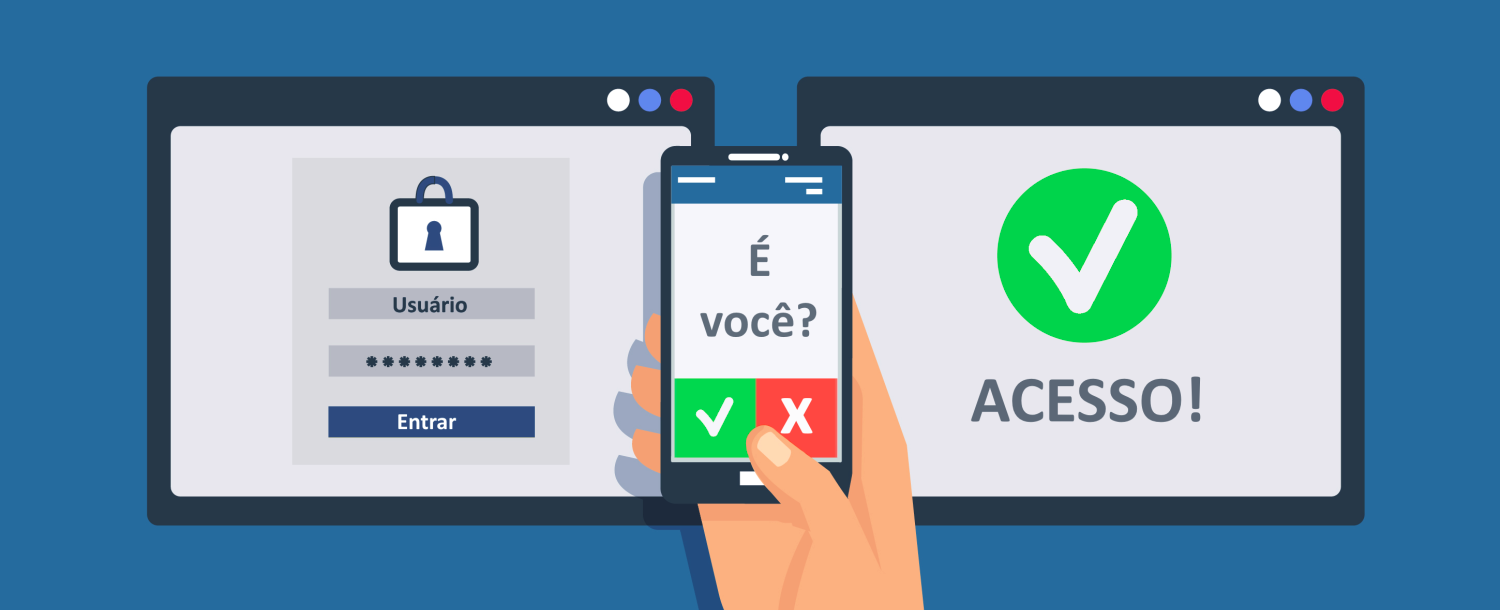
\includegraphics[width=\textwidth]{img/multipla_autenticacao.png}
\end{figure}

Considerando a quantidade de ataques e a necessidade da Segurança da Informação de sempre se aprimorar, a forma de autenticação da identidade apenas por senha, ou seja, algo que o usuário sabe. Para trazer maior segurança passou-se a utilizar modos de autenticação combinados. Desse modo se aumenta a segurança de acessos mais sensíveis ,um bom exemplo é uma conta de banco no celular que não utiliza apenas sua senha, ela utiliza também um celular que a pessoa tenha informado e repassa um código de uso único para o número informado. Essa abordagem é realizada por um número cada vez maior de empresas, mas muitas vezes é preciso ser adotado pelo usuário ainda, o que é muito recomendável de ser feito para acessos delicados, como aqueles que realizam acesso a pagamentos e informações sensíveis.
\begin{ficadica}
    Nas aplicações mais importantes é sempre recomendável adicionar pelo menos 2 formas de autenticação diferentes
\end{ficadica}


\section{Criando e Armazenando Senhas}
A partir desta noção de funcionamento de senhas e de algumas maneiras que elas podem ser descobertas, podemos pensar sobre como manter um acesso de autenticação por senha seguro. Primeiro devemos saber como criar uma senha boa. Depois devemos pensar que hoje em dia criamos cada vez mais senhas para uma infinidade de acessos que precisamos realizar, surge então o questionamento de como lembrar de todas as senhas, se elas devem ser diferentes ou não.

\subsection{Criando Senhas}
O modo como se deve escolher uma senha não é uma unanimidade atualmente. Mas á boas dicas do que não se deve fazer ao criar uma senha e o que se deve fazer como pressuposto básico.

\begin{ficadica}
\textbf{Como não se deve fazer uma senha:}
\begin{itemize}
    \item Não use seu próprio nome, ou o nome do usuário
    \item Não use dados pessoais
    \item Não use nomes próprios
    \item Não use uma sequência de caracteres como "123" ou "abc" ou até "qwerty"
\end{itemize}
\end{ficadica}

\begin{ficadica}
\textbf{Dicas para fazer uma senha:}
\begin{itemize}
    \item Utilize Caracteres do alfabeto com letras maiúsculas e minúsculas
    \item Utilize todos os tipos de caracteres: Letras, Números e Caracteres Especiais
    \item Utilize pelo menos 8 caracteres
\end{itemize}
\end{ficadica}

Seguindo estas dicas há caminhos que podem ser tomados na criação de uma senhas: 

Podem ser criadas senhas de modos aleatórios que trazem alta segurança mas uma difícil memorização. Como por exemplo: Lgaao9l1W80jdOS.

Mas também podem ser criadas senhas que não consideram alguns tipos de ataque, como o ataque de dicionário mas possuem segurança por seus tipos de caracteres e tamanho, e trazem uma facilidade melhor para memorizar. Exemplo: Caixa4Fortificada!

\subsection{Armazenando Senhas}

Bom, além da criação das senhas também é importante pensar sobre como se lembrar delas, sendo que cada vez mais se faz a necessidade da criação de diversas contas de acesso diferentes pela internet. Pensando nisso, é uma boa ideia usar a mesma senha em várias contas? Não, essa não é uma boa ideia, pois ocasionalmente as empresas que guardam estes dados sofrem vazamentos de informações permitindo que as senhas dos usuários sejam conhecidas publicamente. Isso não ocorre apenas em empresas pequenas, grandes empresas também já sofreram e podem sofrer com um vazamento destes. O que ocorre quando um grande volume de senhas são vazadas ao público são diversas pessoas mau-intencionadas que tentam usá-las em outros serviços que a pessoa possui conta, muitas vezes conseguindo acesso com esta mesma senha.

\begin{atencao}
Um modo de guardar senha muito utilizado é anotando a senha em um papel em algum lugar da sua área de trabalho. Essa prática é causa um grande risco de alguém pegar sua senha e se passar por você! 

Então, NÃO FAÇA!!
\end{atencao}

\begin{figure}[h]
\centering
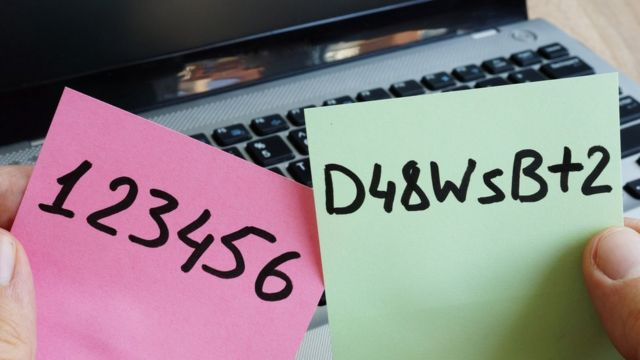
\includegraphics[scale=0.4]{img/Senha_post_it.png}
\end{figure}

Certo, precisamos então fazer uma senha segura e ter uma senha diferente para cada serviço utilizado, como lembrar então de cada senha que tenho? 

O armazenamento de senha é outro problema a ser solucionado para uma Segurança da Informação Pessoal eficiente hoje em dia. Para isso se recomenda a utilização de um programa seguro de armazenamento de senhas. Estes programas atualmente são fornecidos em diversas formas com diferentes funcionalidades, um bom exemplo é o keepass, um software que guarda e gerencia senhas utilizando criptografia para proteção com implementações em windows, linux, macOs, android e iOs. Mas também há gerenciadores de senhas integrados em navegadores de internet como Chrome ou Firefox, que também podem ser utilizados para esta função.

\section{Resumo}
Neste Capítulo aprendemos sobre as formas de acesso a uma área restrita, sendo a principal delas a senha, vimos como funcionam as senhas, como criá-las e como armazená-las. Ainda vemos como tem formas de acesso mistas e que usando isso a nossa segurança fica melhor ainda.

\chapter{Atividades}

\begin{enumerate}
\item Entre no site \href{https://www.security.org/how-secure-is-my-password/} e veja quanto tempo um hacker levaria para descobrir sua senha usando os meios que explicamos nesse capítulo e outros mais sofisticados também.
\item Faça o mesmo teste com a senha de pessoas da família e amigos, você pode até competir para ver quem tem a senha mais segura.
\item Baixe alguma versão do keepass e experimente guardar algumas de suas senhas no aplicativo.
\item Procure alguma conta sua que suporte multiplas formas de de acesso e ative mais de uma forma de acesso.
\item Acesse uma conta sua  em outro dispositivo, veja se há alguma forma de proteção automática quando você acessa sua conta em outro dispositivo.
\end{enumerate}

\part{Ataques Comuns}


\section{Introdução do Capítulo}

Neste capítulo vamos falar sobre os principais ataques virtuais que são realizados contra pessoas, não contra empresas. Conhecendo estes ataques vamos falar também sobre como é possivel se proteger e tentar não ser alvo deles.

\chapter{Ataques comuns}

Depois de entender o valor de suas informações e que você deve protegê-las. E também depois de entendermos sobre o que são formas formas de autenticação e como elas funcionam. Devemos agora entender quais são alguns dos ataques comuns às nossas informações e como devemos nos precaver e não nos expormos a estes ataques.

Entre estes ataques há diversos tipos, muitos deles tem apenas empresas como alvos. Estes são ataques que não podemos impedir. Porém há também ataques que tem como alvo pessoas comuns, neste capítulo vamos nos concentrar nestas ameaças e como é possível ficar atento e se prevenir de alguns destes ataques.

\section{Phishing}

\includegraphics[width=\textwidth]{img/phishing.png}
Phishing, que é um termo como Fishing, pescando em inglês, porém a grafia diferente é utilizada paenas para a ameaça social. Esta é uma das técnicas de ameaça virtual que utiliza Engenharia Social, ou seja, um Hacker atacante se utiliza de uma análise social da vítima para tirar proveito dela e atacá-la. O Phishing traz alguma forma de enganação para a vítima clicar em um link controlado pelo atacante para uma futura ação.

\begin{ficadica}
Esta é uma ameaça de entrada para futuras ações que o atacante utlizará para prejudicar a vítima.
\end{ficadica}

Por se tratar de uma técnica de Engenharia Social e muitas vezes ser passada através de email, a prevenção deste ataque é apenas de cautela. Sempre deve-se ficar atento quando um link para algum acesso delicado é fornecido, algum tipo de banco ou site de comercio online, estes ataques sempre vão se renovando e se sofisticando. A principal chave para não ser enganado é conferir as informações e elementos de mensagem com os meios oficiais de quem envia, ficando atento se a mensagem se mostra ser de fato profissional, muitas vezes as mensagens falsas possuem designs diferentes ou erros de ortografia.

\section{Spoofing}

O Spoofing é uma prática de Fraude, porém no meio digital. Ele pode ser realizado de diversas formas e visa confundir uma vítima passando uma criação de um Hacker atacante como se fosse algo original, podendo ocorrer em sites, aplicativos, emails e mensagens.


\includegraphics[width=\textwidth]{img/spoofing.png}

Emails de Spoofing são muito comuns e trazem uma aparência próxima à mensagens autênticas. Tais mensagens podem ocultar links de Phishing ou então programas maliciosos como Spywares, vírus, worm, entre outros.

Além dos emails, também há o spoofing em sites. Os Hackers utilizam nomes de sites muito parecidos com os originais porém com conteúdos feitos por eles podendo assim adquirir dados sensíveis como senhas de algum cliente enganado pela ameaça.


\section{Spyware}
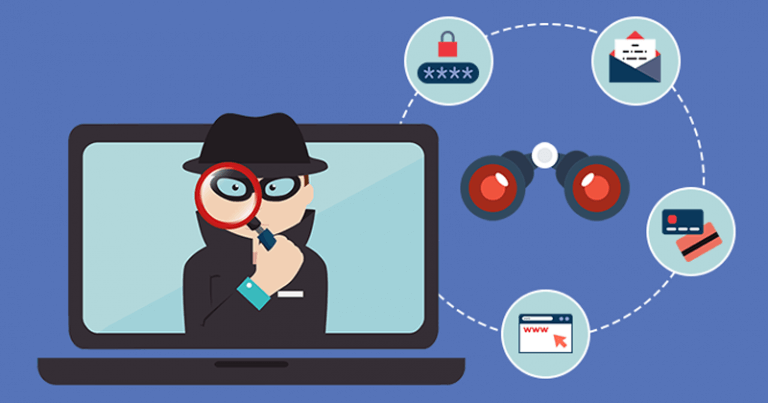
\includegraphics[width=\textwidth]{img/spyware.png}
Spyware, nome que vem de Software Espião, é um tipo de ameaça que registra informações pessoais de algum computador ou celular e passa essas informações para o criador do Spyware. Este registro de informações pode ser realizado de diversas formas, como o keylog que registra apenas os botões acionados pelo usuário, o screenlog que registra tudo o que aparece na tela da vitima da ameaça. A ameaça é perigosa quando o usuário acessa programas ou dados sensíveis, podendo revelar senhas ou dados de acesso restrito para o atacante por meio do programa instalado na máquina.

O Spyware normalmente entra num aparelho a partir de métodos como os explicados acima, phishing ou spoofing podem ser meios para um hacker adicionar um spyware no computador. O primeiro método de proteção é ficar atento a etas ameaças. Porém é sempre importante ter um anti-virus que pode detectar a presença de um destes softwares maliciosos em seu aparelho e retirá-lo.

\begin{atencao}
Uma ferramenta confiável pra descobrir se o site é autêntico é a certificação digital. Este é o cadeado no lado esquerdo do do campo de url, é possível clicar nele e averiguar mais sobre a identidade do site
\end{atencao}

\section{Resumo}
Nesse capítulo estudamos algumas ameaças concretas que podem atacar a segurança da informação pessoal e como nos prevenir delas. Foram elas: Phishing, Spoofing e Spyware.bÉ importante ter esse conhecimento e aplicar suas prevenções sempre no dia a dia.


\chapter{Exercícios}

\subsection*{Exercício 1}

O que é engenharia social e como ela perigosa para a segurança da informação?

\subsection*{Exercício 2}

Quais são as melhores medidas para não ser vítima de ameaças de segurança da informação pessoais?


\part{Bibliografia}
\printbibliography

\end{document}
